\section{Output Compare \& Input Capture}

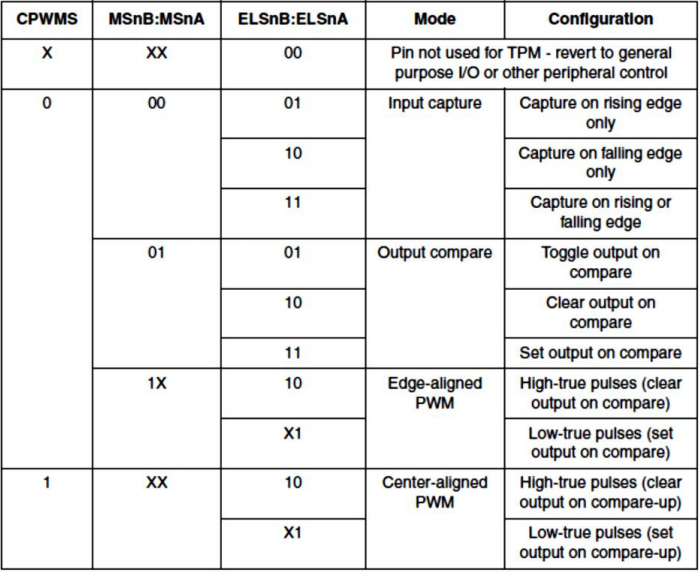
\includegraphics[width=0.5\textwidth]{timer-configuration.png}

\subsection{Timer with Output-Compare}

\textit{
    interrupt is occuring, when the content of the V-Register and
    of the counters have the same value.
}

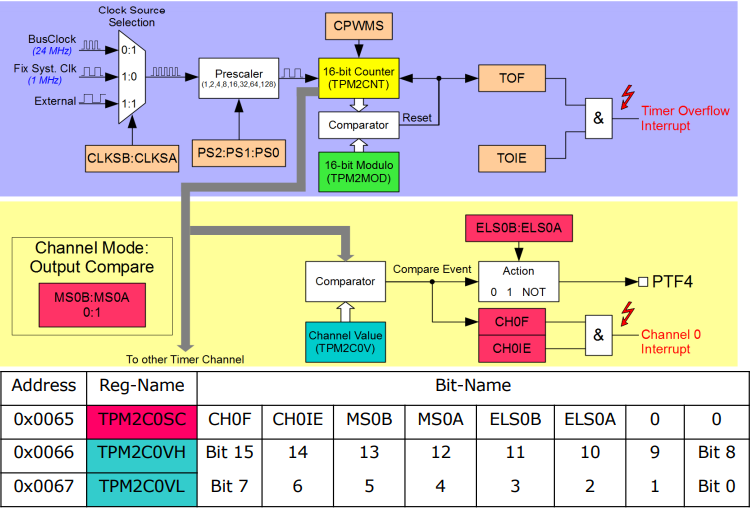
\includegraphics[width=0.5\textwidth]{timer-output-compare.png}

\begin{lstlisting}
void initTimer(void){
    TPM1C1SC_CH1IE = 1; //Channel 1 Timer 1 Interrupt enable
    TPM1C1SC_MS1A = 1; //A=1 ; B=0 - Output Compare
    TPM1C1SC_MS1B = 0;
    TPM1C1SC_ELS1A = 1; //A=1 ; B=0 - Toggle Output on Compare
    TPM1C1SC_ELS1B = 0;
    TPM1C1V = 0x95FF; //set 16bit channel value
    // (is compared with main timer, calc the timer on the base of the clock)
}
interrupt void ISR_outCompare(void){
    TPM1C1SC_CH1F = 0 ; //Timer 1 Channel 1 overflowflag reset
    TPM1C1V += 0x95FF ; //Channel Value is set to new value
    // (add with the value, on how much time needs to pass)
}
\end{lstlisting}

\subsection{Usage Output Comapre Mode}

\textit{
    The output compare mode can be used to setup
    different timers on base of the same timer wihout
    changing the TPMxMOD value.
}

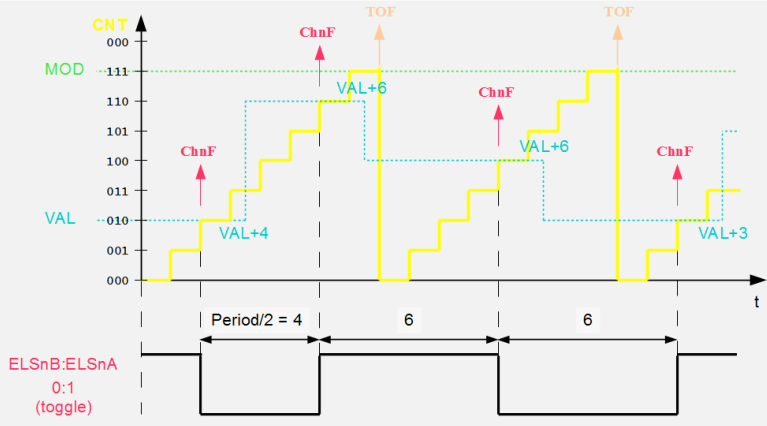
\includegraphics[width=0.5\textwidth]{output-compare-timer-trick.png}

\subsection{Input Capture}

\textit{
    Input capture is used on the timer pins. it enables
    reacting on input (rising/falling or both).\newline
    If an input capture happens, the interrupt is
    executed and the current counter is saved in the channels
    value register for further usage.
}


